\section{Theoretical foundations}
In order to understand the rather peculiar properties of semiconductors, we will first give
a short introduction into the theory of bonds and bands, following \cite{phillips2012bonds}.
Let us consider an assembly of $N$ atoms forming a crystal, each with its discrete energy level $E_\alpha$.
we will now denote the average spacing of atomic levels with $\Delta E_\alpha$. As we narrow the distance
between the atoms, the electrons originally bound to the attractive potential of one nucleus begin to interact
with the potentials of other nuclei. This shifts each energy level $E_\alpha$ and eventually the formerly
discrete levels become bands of levels with an energy spacing of order
\begin{equation}
    \delta = \Delta E_\alpha / N
\end{equation}
while the spacing $\delta$ becomes negligible when it is much smaller then $kT$, because 
of the thermal fluctuations. Thus at room temperature a collection of several hundred atoms
at solid densities behaves in many repects like solid. The electrons are then distributed among these
energy levels according to the pauli exclusion principle with the probability
\begin{equation}
    P = \frac{2}{\exp \left [(E_n - E_F)/ kT  + 1\right ]}
    \label{eq:fermidist}
\end{equation}
with the fermi energy, which is in the 3d isostropic, non-interacting fermi gas
\begin{equation}
    E_F = \frac{\hbar^2  }{2m} \left ( \frac{3 \pi^2 N}{V} \right )^{2/3}
\end{equation}
with volume $V$ and single electron mass $m$. For $E_F \gg kT$ equation \eqref{eq:fermidist} corresponds
to a step function with one for $E < E_F$ and zero for $E > E_F$. While this intuitive explanation gives
an idea where how bands from energy levels emerge, it does not explain the huge gap between these bands
in, for instance, insulators. We cannot rely on the single atom - electron theory alone in order to understand
this phenomenon, we have to consider the emergent property of the solid itself, therefore we will 
give a short introduction into blochtheory.
\subsection{Blochtheory}
Blochtheory does very general statements about wavefunctions of particles in periodic potentials and
yields hence a model for explaning the band structure in solids.
We can write down the Schrödinger equation for an electron without interaction as 
\begin{equation}
    \hat{ H} \psi(\R) = \left [ - \frac{\hbar^2}{2m} \Delta + V(\R) \right] \psi(\R) = E \psi(\R)
\end{equation}
with periodic potential
\begin{equation}
    V(\R) = V(\mathbf{r + r_n}); 
\qquad \mathbf{r_n} = n_1 \mathbf{a_1} + n_2 \mathbf{a_2} + n_3 \mathbf{a_3} 
\end{equation}
where the lattice vectors $\mathbf{a_i}$. Because of its periodicity we can develop the
potential in a fourier series:
\begin{eqnarray}
    V(\R) &= &\sum_\G \VG \mathrm{e}^{i\G \cdot \R} \\
    \mathrm{mit \ Fourierkomponente \quad}  \VG &= &\frac{1}{L} \int \mathrm{e}^{i\G \cdot \R} 
    V(\R) \mathrm{d}\R  \nonumber \\
    \mathrm{und \ reziprokem \ Gittervektor \quad} \G &= &h\mathbf{g_1} + k\mathbf{g_2} +l\mathbf{g_3}; 
    \quad h, \ l, \ k, \ \in \mathbb{Z}. \nonumber
\end{eqnarray}
The ansatz for a solution is a linear combination of plane waves
$ \psi(\R) = \sum_\K C_\K \mathrm{e}^{i\K \cdot \R}, $
which have to fullfill
\begin{equation}
    \sum_\K \mathrm{e}^{i\K \cdot \R} 
    \Big[ \Big( \frac{\hbar^2 k^2}{2m} - E\Big) C_\K + \sum_\G \VG C_{\K - \G}\Big] 
    = 0.
\end{equation}
Linear independence of $\R$ leads to
\begin{equation}
    \Big( \frac{\hbar^2 k^2}{2m} - E\Big) C_\K + \sum_\G \VG C_{\K - \G}= 0
\end{equation}
For every $\K$ value we have $N$ equations, which couple the coefficients $C_\K$ respectively with 
$C_{\K - \G'}$, $C_{\K - \G''}$,\ldots, where $N$ is the number of elementary cells of the lattice.
The wave functions of energy  $E_\K$ can thus be written as superposition of plane waves, whose 
$\K$ vectors lay on the reciprocal lattice:

\begin{eqnarray}
    \psi_\K(\R)&=& \sum_\G C_{\K - \G} \mathrm{e}^{i(\K - \G) \cdot \R} \nonumber \\
            &=& \sum_\G C_{\K - \G} \mathrm{e}^{i \G \cdot \R}  \mathrm{e}^{i\K \cdot \R} \nonumber \\
            &=& u_\K(\R) \cdot \mathrm{e}^{-i\K \cdot \R} 
\end{eqnarray}
Those wavefunctions we call \textbf{Bloch waves}.
The bloch theorem yields for the one electron problem in the periodic potential those bloch waves 
as energy eigenfunctions with the eigenvalues
$E_\K$ with $\K = \frac{2 \pi}{L} (n_x, n_y, n_z)$ and
\begin{equation}
    u_\K(\R) = u_\K(\mathbf{r + r_n}) .
\end{equation}
We can conclude that
\begin{equation}
    \psi_{\K + \G}(\R) = \psi_\K(\R) 
\end{equation}
and equivalently 
\begin{equation}
    E(\K) = E(\K + \G).
\end{equation}
For the probabability distribution we have $|\psi(\mathbf{r})|^2 = |u|^2$ --  
We can take hence the electron density as measured variable for the positions of the atoms.
Assuming a quasi free electron the bloch theory leads to assumptions about the band structure in solids.
Let us assume a free electron in periodic space. Shifting the reciprocal lattice by $\G$ we can
write down the schrödinger equation as follows
\begin{eqnarray}
    \Big(E - \frac{\hbar^2}{2m}|\K - \G|^2\Big) C_{\K - \G} &=&
        \sum_{\G'} V_\mathbf{G' - G} C_{\K - \G'}, \quad \mathrm{d.\ h.} \nonumber \\
    \label{eqn:bloch1}    
    C_{\K - \G} &=& \frac{ \sum_{\G'} V_\mathbf{G' - G}}{E - \frac{\hbar^2}{2m}|\K - \G|^2} 
\end{eqnarray}
Perturbing the free electron, we can express the energy in first order still by
$E = (\hbar^2 k^2) / (2m)$. Since only the biggest terms of $C$ contribute, this
means in return that the denominator is small in \eqref{eqn:bloch1}. This is the same
as saying that the condition
\begin{equation}
    E(\K) = E(\K + \G)
\end{equation}
is fulfilled for huge $C$, which is the condition for bragg reflection, i.e. the biggest 
deviations compared to the free electron occur, when the $\K$ Vektor is at the border of the
so called \emph{1. Brillouin zone} .
Furthermore, plugging $\G = 0$ in \eqref{eqn:bloch1} yields $V_0 = 0$, which leads to the assumption that
$C_\K$ is contributing even in first order. Hence we get the system of equations 
\begin{eqnarray}
    \psi_\K(\R)&=& \sum_\G C_{\K - \G} \mathrm{e}^{i(\K - \G) \cdot \R} \nonumber \\
            &=& \sum_\G C_{\K - \G} \mathrm{e}^{i \G \cdot \R}  \mathrm{e}^{i\K \cdot \R} \nonumber \\
            &=& u_\K(\R) \cdot \mathrm{e}^{-i\K \cdot \R}
\end{eqnarray}
which can be solved in terms of the determinant equation
\begin{eqnarray}
    \begin{vmatrix}
        \Big(\frac{\hbar^2}{2m} k^2 - E\Big) & \VG \\
        V_\mathbf{-G}   & \Big(\frac{\hbar^2}{2m} |\K - \G|^2 - E\Big) 
    \end{vmatrix} = 0; \\
    E_{\K - \G}^0 := \frac{\hbar^2}{2m} |\K - \G|^2 \nonumber
\end{eqnarray}
with the solutions
\begin{equation}
    E^\pm = 
    \frac{1}{2}(E_{\K - \G}^0 + E_\K^0) \pm 
        \frac{1}{2}\Big[(E_{\K - \G}^0 + E_\K^0)^2 + |\VG|^2\Big]^{\frac{1}{2}}.
\end{equation}
At the border of the first Brillouin zone we have hence  $E_{\K - \G}^0 = E_\K^0$. 
This yields for the energy differences between the bands:
\begin{equation}
    \Delta E = E^+ - E^- = 2 |\VG|.
\end{equation}
For the one dimensional case, refer to figure~\ref{fig:bloch} for a visualization
\cite{ibach2009festkorperphysik}.

\begin{figure}[!t]
  \begin{captionbeside}[]{
          Visualization of the split-up of the energy parabela of the free electron (dashed)
          at the border of the first Brillouin zone and in the case of a perturbationtheoretic
          consideration of electrons in the periodic lattice, with the bands (1) and (2),
obtained from \cite{ibach2009festkorperphysik}.}[r]
    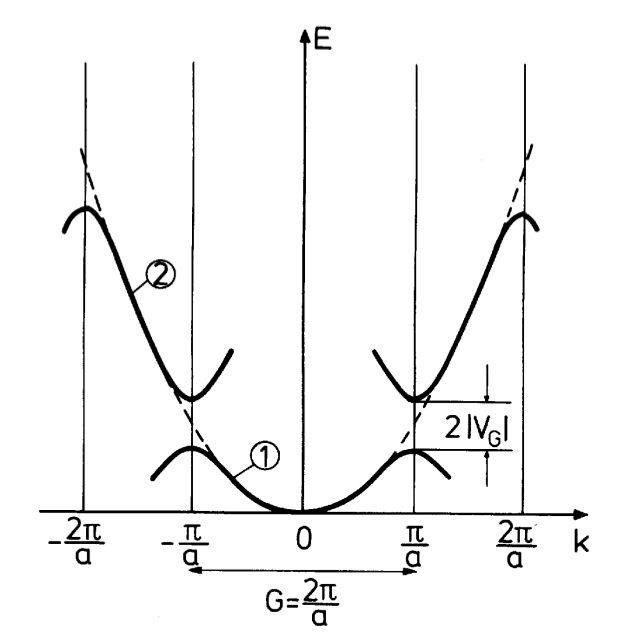
\includegraphics[width=0.5\textwidth]{figures/bloch}
  \end{captionbeside}
  \label{fig:bloch}
\end{figure}
\newpage
In a real crystal we have to consider several deviations from the previous model:
\begin{enumerate}
    \item Crystals have a finite size as we have considered in the introduction. Therefore
        we cannot start from the free electron solution, but have to include discrete energy 
        levels from the beginning, which coming from the stated aspects, broaden.
    \item The broadening comes amongst other reasons from the electron-electron and 
        electron-phonon interaction. We assumed this to be neglectible small, but even
        the small interaction leads to the overlap of several energy levels, creating
        the already introduced bands, see figure~\ref{fig:baender1}.
\end{enumerate}
For each band we have to incorporate the pauli principle with for electrons two spin directions.
For temperatures going to zero, the electrons are distributed in the lowest energy levels, as in
equation ~\ref{eq:fermidist}. The lowest energy band below the fermi energy is called
\emph{valence band}, since the electrons are bounded in a way that we cannot have a current.
The band above the fermi energy is called the \emph{conduction band}, since electrons can surpass their
localized state and with sufficient energy change their expection value of position with an applied
exterior field.
\begin{itemize}
    \item Metals are conducting, because the valance band and the conduction band overlap and 
        free electrons exist even without applying an exterior field.
    \item For isolators the band gap is huge compared to the fermi energy, hence it is not probable for
        the electrons to surpass this gap.
    \item The conductance in semiconductors is dependent on the energy brought in, for instance they
        are sensitive to the temperature, because the fermi energy is between the valance and the
        conduction band. Up from a certain applied exterior field electrons can shift to energies
        higher than the lowest energy of the conduction band -- a current can flow.
\end{itemize}

See figure~\ref{fig:baender2} \cite{demtroder2000experimentalphysik}\\ for
a visualization of these concept.
In our experiment we will use silicon (Si) and germanium (Ge). 
Both are intrinsic semiconductors, which means that the property of semiconduction is not 
driven through dotation, but by the intrinsic properties of the solid.
\subsection{Indirect and direct semiconducters}
In the former theory we simplified the scenario to a great extent, but in reality many 
different specifications of the concept are possible. One important concept is the existence
of direct and indirect band gaps: The ones which we looked at before were all direct band gaps, such
that only a specific energy is necessary to surpass the energy gap. Indirect band gaps require additionally 
a nonzero change of the momentum, which in principle origins in most cases from interaction with a phonon.
The momentum before and after the transformation to the conduction band is hence finite, implying
a further constraint to the creation of electron-hole pairs. As result a photon with an energy close to
the band gap is less likely to be absorbed in an indirect band gap than in a direct one. \\
For our experiment it is relevant that silicium is an indirect semiconductor while germanium is a direct one. 

\newcommand{\picwidththeo}{0.48\textwidth}

\begin{figure}
    \centering
    \begin{subfigure}[b]{\picwidththeo}
        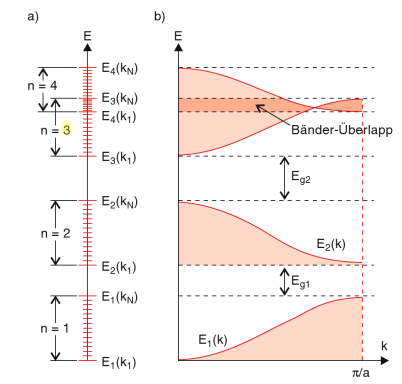
\includegraphics[width=\textwidth]{figures/baender1}
        \caption{ Creation of energy bands. We see the split-up of the
            allowed energy values of $N$ electrons in a crystal.
            (a) one dimensional visualization,
            (b) visualization of $E_n(k)$, with the 1. Brillouin zone (dashed) from
}
        \label{fig:baender1}
    \end{subfigure}\qquad
    \begin{subfigure}[b]{\picwidththeo}
        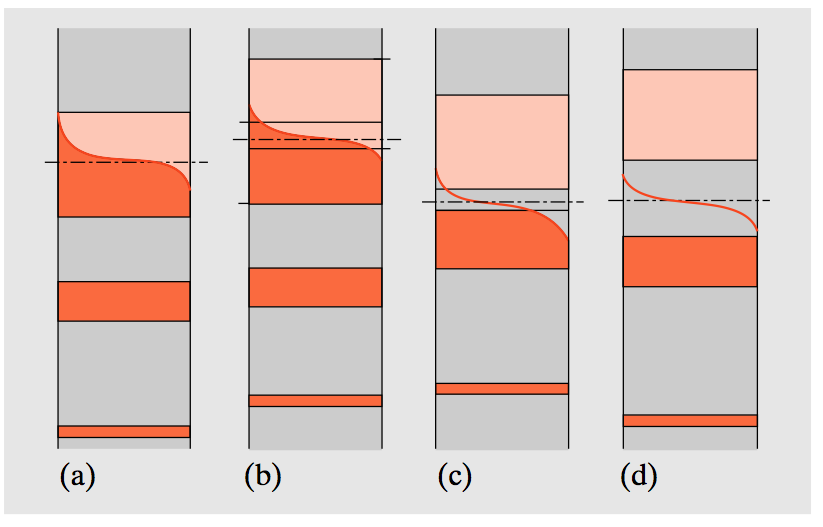
\includegraphics[width=\textwidth]{figures/baender2}
        \caption{Schematic visualization of the band structure for
            (a) metals of the first main group (alkaline),
            (b) metals of the second main group  (alkaline earth metal), 
            (c) semiconductor (in the conducting phase),
            (d) isolators.
            Obtained from \cite{vogel1997gerthsen}.}
        \label{fig:baender2}
    \end{subfigure}
    \caption{Band structure in solids}
    \label{fig:baender}
\end{figure}

\section{Interaction of photons with matter}
We will exploit a particular effect only possible within the description of quantum mechanics, the
photoelectric effect\footnote{Despite the fact that Heinrich Hertz discovered the 
photoeletric effect already in 1887, it was not possible to explain it until Albert Einstein
published an explanation 1905 with which he shows the quantum character
of light. 1921 he was rewarded with the Nobel Price in physics.}. 
Whether the photon is interacting with an electron depends on its energy
\begin{equation}
    E_\gamma = h \nu.
\end{equation}
Only when surpassing the bounding energy of the electron the photon will have an effect. In that
case the electron will be quasi free, leaving a hole behind, which in return will be refilled with
an electron of a higher shell by emitting a photon (in principle also the creation of Auger electrons is
possible, such that no photon is created). 




\begin{equation}
    c(t, x) = C \cdot \frac{1}{\sqrt{4 \pi D_n t}} 
    \cdot \exp\left( -\frac{\left( x - \mu_n E t \right)^2}{4 D_n t} \right)
    \label{eq:c_t_x}
\end{equation}

